% Section 5: Reading labels and data product files

\section{Reading labels and data product files}
\label{sec:reading-labels-and-data-product-files}


\subsection{Introduction}
\label{sec:introduction-2}

The files in this bundle are archived in PDS4 format. PDS4 has the following basic structure:

\begin{itemize}
\item A \textit{bundle} consists of one or more \textit{collections}
\item A \textit{collection} consists of one or more \textit{data products}
\item Each \textit{data product} is defined by PDS4 label (\code{.\allowbreak{}lblx}), which gives information about the data and also includes information about the additional associated files that contain the actual data. These data files may be binary or text and may be stored in a variety of formats.
\end{itemize}
A full discussion of the PDS4 format is beyond the scope of this document and readers are referred to the resources in Section \ref{sec:pds4-standards-and-documentation} for additional reading. However, we will endeavor to provide enough information here to allow reading of these various files for research purposes without comprehensive knowledge of the PDS4 standard.

Two types of software can be used to read PDS4 labels and data files: generic off-the-shelf software that doesn’t understand PDS4 concepts, and specific tools or programming libraries that understand PDS4 labels. We will start by discussing the former.


\subsection{Using off-the-shelf programs}
\label{sec:using-off-the-shelf-programs}

Label files (\code{.\allowbreak{}lblx}), table files (\code{.\allowbreak{}tab}), and CSV files (\code{.\allowbreak{}csv}) are standard text files that can be read with any text editor. However, while this is sufficient to give you an overview of the contents of the file, each file has a specific format designed to be read and parsed by specific types of programs, and this can be done without the need for PDS4-specific software. Using the correct program in the correct way will make using these files much easier and more productive.


\subsubsection{Label files}
\label{sec:label-files}

Label files are written in XML (eXtensible Markup Language), a hierarchical file format much like a nested outline. For the best results, the use of a text editor that understands XML is helpful. Such an editor will likely have two main features:

\begin{itemize}
\item The ability to collapse and expand different levels of the hierarchy, so as to hide parts of the label that aren’t needed for the task at hand; and
\item Syntax coloring, where the open and close tags (\code{<tagname>data</\allowbreak{}tagname>}) are color-coded for ease of identification.
\end{itemize}
As text editors are constantly coming in and out of favor and are platform-specific, we will not recommend specific tools here. However, almost every sophisticated editor or programming IDE (Integrated Development Environment) either natively supports XML or has an XML plugin. In most cases the editor will automatically recognize the file as being in XML format, but in some cases it might be necessary to explicitly invoke the XML mode if the editor relies on the file extension (since \code{.\allowbreak{}lblx} is not a normal XML extension).


\subsubsection{Table files}
\label{sec:table-files}

Files with the extension \code{.\allowbreak{}tab} (including the metadata parameters, source image index, and global indexes) are formatted as \textit{fixed-width comma-delimited tables}. That is, they look like:

\begin{CodeBlock}
Value123   ,ValueA  ,ValueB
Value45678 ,ValueCDE,ValueF
\end{CodeBlock}

This format allows software that knows the width of each column to efficiently read the table (see below), but simultaneously permits reading by the wide range of software that supports comma-separated value (CSV) files, such as spreadsheet programs. In this case, when opening the table file, you may find that the program identifies the table as fixed-width. Unfortunately, in this case, it will end up adding the comma to each field. To properly read a table in a spreadsheet program, be sure to specify that the file is “delimited” and that the delimiter is “,”; also specify that you want whitespace stripped if possible.


\subsubsection{CSV files}
\label{sec:csv-files}

Files with the extension \code{.\allowbreak{}csv} (mainly the collection files) are formatted as \textit{variable-width comma-separated value} files. These files can be read the same way as the above table files, except it is more likely programs will correctly identify them as delimited instead of fixed width from the beginning.


\subsubsection{Image files}
\label{sec:image-files}

Files with the extension \code{.\allowbreak{}img} hold the reprojected images and mosaics. They are raw binary arrays with no header, no record separators, and no padding: LSB (little-endian) IEEE 754 single-precision floats, with the longitude index varying fastest so that the data reshapes directly to 401 radii by \textit{N} longitudes, and with the value −999 marking any element that has no valid data (Section \ref{sec:data-reproj-img}).
The example programs described in Section \ref{sec:example-programs} demonstrate how to read and display these files.


\subsection{Using PDS4-specific software}
\label{sec:using-pds4-specific-software}

A variety of software is available for reading PDS4-format data. Note that over time tools evolve and are replaced, and the URLs or package names where tools can be found change. This section includes tools and their locations at the time of publication. To find new or updated tools, use the resources in Section \ref{sec:pds4-standards-and-documentation}.


\subsubsection{The Small Bodies Node tools}
\label{sec:the-small-bodies-node-tools}

The PDS Small Bodies Node (SBN) has a variety of software useful for reading PDS4-format data. This includes:

\begin{itemize}
\item \textbf{PDS4 Viewer}: This standalone application is capable of reading PDS4 labels and associated tabular and binary data files and displaying them in various formats. \newline \href{https://pds-smallbodies.astro.umd.edu/tools/pds4_tools_info/pds4_viewer.html}{https://pds-smallbodies.astro.umd.edu/tools/pds4\_\allowbreak{}tools\_\allowbreak{}info/pds4\_\allowbreak{}viewer.html}
\item \textbf{Python PDS4 Tools}: This Python module will read and display PDS4 labels and associated tabular and binary data files. The read data can easily be used in Python programs for further analysis.\newline \href{https://pdssbn.astro.umd.edu/tools/pds4_tools_info/python_pds4_tools.html}{https://pdssbn.astro.umd.edu/tools/pds4\_\allowbreak{}tools\_\allowbreak{}info/python\_\allowbreak{}pds4\_\allowbreak{}tools.html}
\item \textbf{ReadPDS}: This IDL module will read and display PDS4 labels and associated tabular and binary data files. The read data can easily be used in IDL programs for further analysis.\newline \href{https://pdssbn.astro.umd.edu/tools/tools_readPDS.shtml}{https://pdssbn.astro.umd.edu/tools/tools\_\allowbreak{}readPDS.shtml}
\end{itemize}

\subsubsection{The Ring-Moon Systems Node tools}
\label{sec:the-ring-moon-systems-node-tools}

The PDS Ring-Moon Systems Node (RMS) provides a Python PDS4 table reader that can also fetch tables from remote locations. It is based on the SBN PDS4 label reader.\newline \href{https://rms-pdstable.readthedocs.io/en/latest/}{https://rms-pdstable.readthedocs.io/en/latest/}


\subsubsection{The Planetary Data Reader}
\label{sec:the-planetary-data-reader}

The Planetary Data Reader (PDR) is a Python package that endeavors to be able to read all PDS3 and PDS4 format data with a uniform interface. PDS4 support is based on the SBN PDS4 label reader.\newline \href{https://pdr.readthedocs.io/en/latest/}{https://pdr.readthedocs.io/en/latest/}


\subsubsection{Example programs}
\label{sec:example-programs}

The F ring bundle includes example Python programs explicitly designed for reading and manipulating the mosaic and reprojected image data products. Each program is thoroughly commented to aid the user in learning the concepts involved. The programs can be found in the \code{document/\allowbreak{}user\_\allowbreak{}guide} directory (Section \ref{sec:user-guide}).

\begin{itemize}
\item \textbf{mosaic\_\allowbreak{}utils.py}:\textbf{ }A support module that is used by all other example programs and that can be directly imported into user-developed programs. It supplies the following functions:
\begin{itemize}
\item \textbf{get\_\allowbreak{}element}: Search a label for a particular element name and return its value.
\item \textbf{contrast\_\allowbreak{}stretch}: Non-linearly stretch an image based on blackpoint, whitepoint, and gamma values.
\item \textbf{read\_\allowbreak{}mosaic\_\allowbreak{}ma }and \textbf{read\_\allowbreak{}reproj\_\allowbreak{}img\_\allowbreak{}ma}: Read an F ring mosaic or reprojected image into a numpy masked array with the metadata returned as a structured numpy array.
\item \textbf{read\_\allowbreak{}mosaic\_\allowbreak{}ma\_\allowbreak{}df }and \textbf{read\_\allowbreak{}reproj\_\allowbreak{}img\_\allowbreak{}ma\_\allowbreak{}df}: Read an F ring mosaic or reprojected image into a numpy masked array with the metadata returned as a pandas DataFrame.
\item \textbf{get\_\allowbreak{}mosaic\_\allowbreak{}name\_\allowbreak{}from\_\allowbreak{}lid} and \textbf{get\_\allowbreak{}reproj\_\allowbreak{}img\_\allowbreak{}name\_\allowbreak{}from\_\allowbreak{}lid}: Convert a LID to the name of the mosaic or reprojected image.
\item \textbf{get\_\allowbreak{}mosaic\_\allowbreak{}name\_\allowbreak{}from\_\allowbreak{}mosaic\_\allowbreak{}label} and \textbf{get\_\allowbreak{}reproj\_\allowbreak{}img\_\allowbreak{}name\_\allowbreak{}from\_\allowbreak{}label}: Get the name of the mosaic from the mosaic label or the name of a reprojected image from the reprojected image label.
\item \textbf{get\_\allowbreak{}mosaic\_\allowbreak{}name\_\allowbreak{}from\_\allowbreak{}reproj\_\allowbreak{}img\_\allowbreak{}label}: Get the name of the mosaic that incorporates a reprojected image from the reprojected image label.
\item \textbf{read\_\allowbreak{}index\_\allowbreak{}np}: Read a global index into a numpy array.
\item \textbf{read\_\allowbreak{}index\_\allowbreak{}df}: Read a global index into a pandas DataFrame.
\end{itemize}
\item \textbf{display\_\allowbreak{}reproj\_\allowbreak{}img.py: }Display a single reprojected image.
\item \textbf{plot\_\allowbreak{}ews\_\allowbreak{}ma.py: }Plot a mosaic along with its equivalent width profile using numpy masked arrays for computation.
\item \textbf{plot\_\allowbreak{}ews\_\allowbreak{}df.py: }Plot a mosaic along with its equivalent width profile using pandas DataFrames for computation (same functionality as the previous program, but the internals are different for illustration).
\item \textbf{find\_\allowbreak{}prometheus\_\allowbreak{}closest\_\allowbreak{}approaches.py: }Search the global reprojected image index file for images where Prometheus is visible and display the 10 images where Prometheus is closest to the F ring core at that time.
\end{itemize}
Here are example uses:

\begin{CodeBlock}
$ python display_reproj_img.py \
    /path/to/bundle/data_reproj_img/iss_036rf_fmovie001_vims/1545564642n_reproj_img.lblx
\end{CodeBlock}

\noindent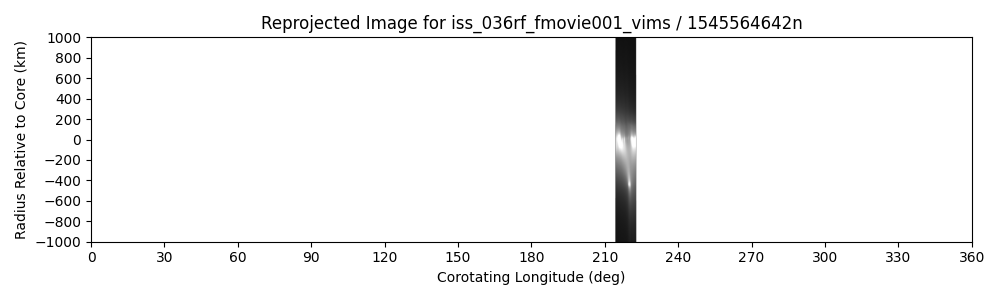
\includegraphics[width=\linewidth]{figures/screenshot-display-reproj-img.png}

\begin{CodeBlock}
$ python plot_ews_ma.py \
    /path/to/bundle/data_mosaic_bkg_sub/iss_036rf_fmovie001_vims/iss_036rf_fmovie001_vims_mosaic_bkg_sub.lblx
\end{CodeBlock}

\noindent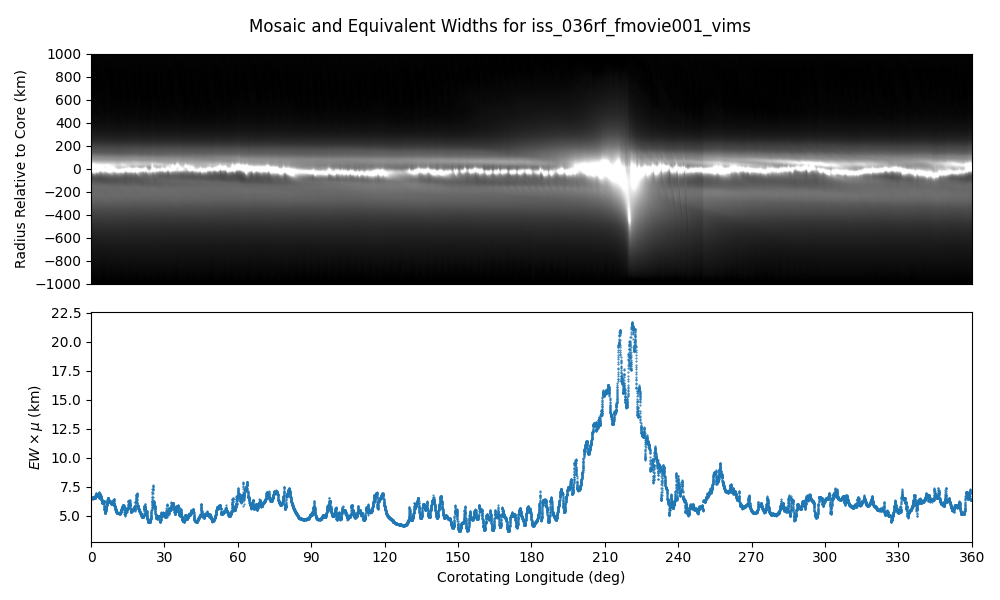
\includegraphics[width=\linewidth]{figures/screenshot-plot-ews.png}

\begin{CodeBlock}
$ python find_prometheus_closest_approaches.py /path/to/bundle
\end{CodeBlock}

\noindent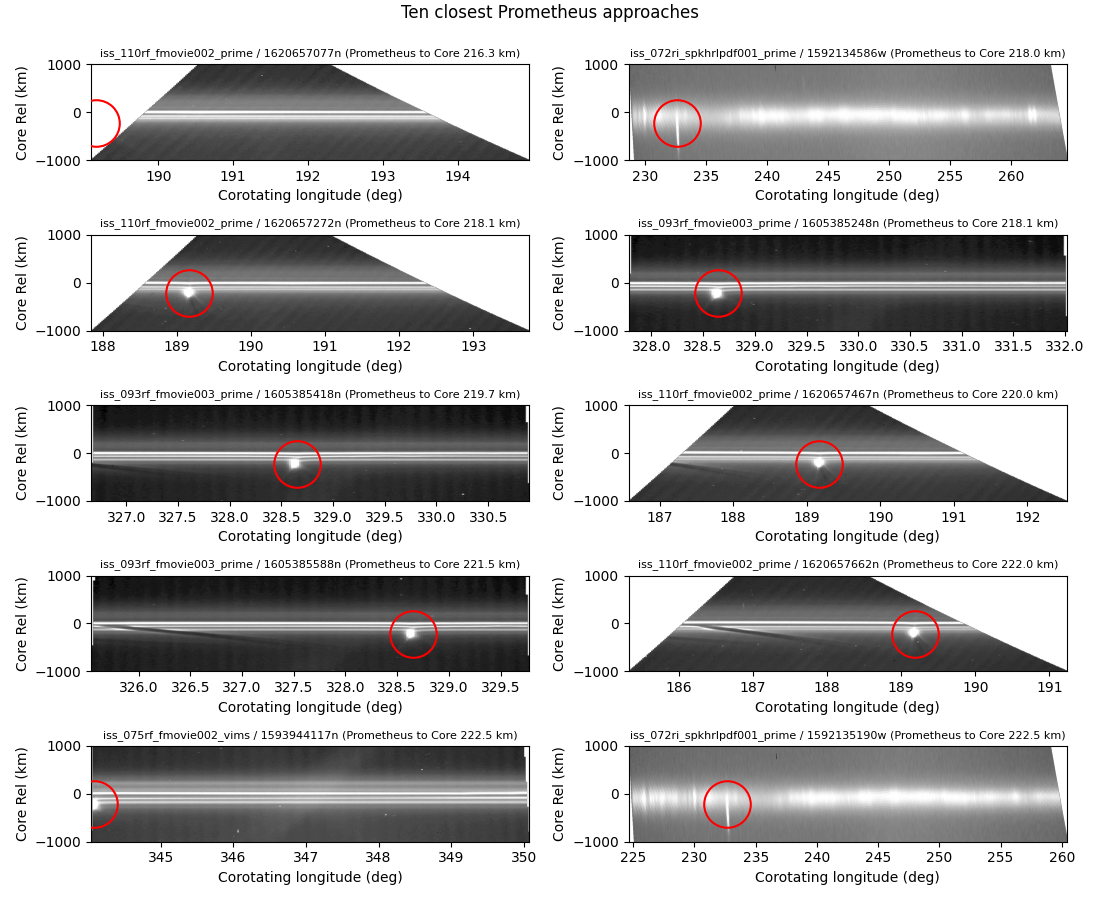
\includegraphics[width=\linewidth]{figures/screenshot-find-prometheus.png}


\subsubsection{F ring bundle analysis programs}
\label{sec:f-ring-bundle-analysis-programs}

In addition to the example programs included with the archived bundle, additional software is available to aid researchers in viewing and analyzing the data. As this software evolves rapidly, it is not included with the bundle, but is instead available in this GitHub repo:

\href{https://github.com/SETI/fring-mosaics-bundle-software}{https://github.com/SETI/fring-mosaics-bundle-software}
